\mtnote{TODO: replace `resource' with `site'; `http' to `HTTP'?}

The design of the Production and Distributed Analysis (PanDA) system started in
2005 to develop a WMS for the ATLAS experiment. PanDA went into production for
the LHC Run 1 on 2009 and was then partially redesigned to be deployed on Run 2,
on 2015. In this section, we summarize the design, architecture, and execution
process of the current state of the practice.


% -----------------------------------------------------------------------------
\subsection{Design}
\label{ssec:panda_design}

% \begin{itemize}
%   \item No MPI tasks?
%   \item Pilot multitenancy?
%   \item PanDA Server Brokerage component and Event service interaction?
%   \item PanDA Server Data Service component and Event Service interaction?
% \end{itemize}

PanDA's application model primarily assumes single tasks, workloads and
workflows. Tasks represent a set of operations performed on a set of events,
stored across input files. Tasks can be decomposed into jobs, where each job
represents the task's set of operations and a partition of the task's events.
Since 2005, a certain amount of parallelism has been progressively introduced
for jobs~\cite{multithreaded_jobs} but, so far, no MPI jobs have been considered
for production. Jobs are supposed to be relatively self-contained, capable of
setting up their own execution environment or having a minimal set of common
dependences. Different types of job payload (i.e., executable) are assumed, both
in terms of user-defined batch scripts or application frameworks for group of
users.

PanDA's user model is based on multitenancy and the support of at least two
types of HEP users: individual researchers and groups executing production-grade
workflows. Users are considered free to submit tasks and workflows to the PanDA
WMS at any point in time, directly or via dedicated application frameworks.
Consistently, PanDA's security model is based on separation between
authentication, authorization and accounting for both single users and group of
users. Both authentication and authorization are based on digital certificates
and the X.509 standard and on the virtual organization abstraction.

Currently, PanDA's execution model is based on five main abstractions: task,
job, queue, pilot, and event. Both tasks and jobs are assumed to have attributes
and states and to be queued into a global queue for execution. Prioritization
and binding of jobs are assumed to depend on the attributes of each job. Pilot
is used to indicate the abstraction of resource capabilities. Jobs are thought
to be bound to pilots and the execution of their payload is performed on the
site where the pilots has been instantiated. Consistently, pilots are considered
to be multitenant as jobs belonging to multiple workflows and/or users can be
bound and executed on them.

PanDA' data model uses events as the unit of data. Each event represents a
collision captured in the detector and one or more events can be packaged into
files or data source with other container abstractions. As with jobs, data have
both attributes and states, and some of the attributes are shared between events
and jobs so to create associations. Raw, reconstruction, and simulation data are
assumed to be distributed across multiple and tiered sites and managed by the
ATLAS Distributed Data Management (DDM)~\cite{garonne2012atlas}. Datasets
required by each job are assumed to be replicated when necessary over the
network. This applies to both input and output data. \sergeynote{Raw data from
the ATLAS detector is captured at CERN and goes through reconstruction step to
produce data in secondary formats, smaller in volume and with more and more
physics content instead of raw detector hits. Consequently a second, custodial,
copy of raw data is being distributed in predetermined volumes to National T1
centers around the world (like BNL  T1 center). This insures low raw data
redundancy and safety. Multiple copies of chunks of secondary data sets (derived
from real raw data) are also distributed to ~100 centers around the word for
ease of access and improved availability for analysis. Then raw detector data is
stored on Tapes at CERN, just  in case. Most users, who do physics analysis,
rarely work with raw data, only a small group of experts needs to work with raw
data for specialized tasks like detector calibrations and such. There may be a
need to redo a reconstruction step, when errors in previous reconstruction
campaign are uncovered or improved detector understanding will lead for a better
quality physics. Then data stored on tape is recovered and re-processed again.
Simulation data is produced in many places anyway and is not centralized to
begin with. Here's the paper that describes current DDM state in ATLAS, data
replication strategies and such.
http://iopscience.iop.org/article/10.1088/1742-6596/396/3/032045/pdf DDM is a
complex and evolving topic in ATLAS.}\mtnote{Thank you. As we are describing the
design of PanDA I thought we should not enter into a too detailed description of
the DDM design. I eliminated the mistake I had made about `centralized data' but
left DDM just as a reference. Any better?}

PanDA design supports provenance and traceability for both jobs and data.
Attributes enable provenance by linking jobs and data items, providing
information like ownership or project affiliation. States enable traceability by
providing information about the stage of the execution in which each job or data
item is or have been. Some attributes are assumed to be immutable across
execution and jobs and data items are assumed to be always in one and only one
state.


% -----------------------------------------------------------------------------
\subsection{Architecture}
\label{ssec:panda_arch}

The implementation of PanDA consists of several interconnected subsystems, most
of them built from off-the-shelf and Open Source components. At a high level,
PanDA's architecture has six main subsystems: PanDA Server, AutoPyFactory, PanDA
Pilot, PanDA Monitoring, JEDI, and Event Service. Subsystems communicate via
dedicated API or http messaging. Databases are used to store eventful entities
like tasks, jobs and events, and to store information about resources, logs, and
accounting. Each subsystems is implemented by one or more modules as shown in
Figure~\ref{fig:architecture}. In the following, we briefly describe the overall
architecture of PanDA and its components. The description provides all the
details required to understand how HPC resources have been integrated within
PanDA (\ref{sec:integration}). For a more detailed description of PanDA
architecture see~\cite{wiki, papers}.

\begin{figure}
  \begin{center}
    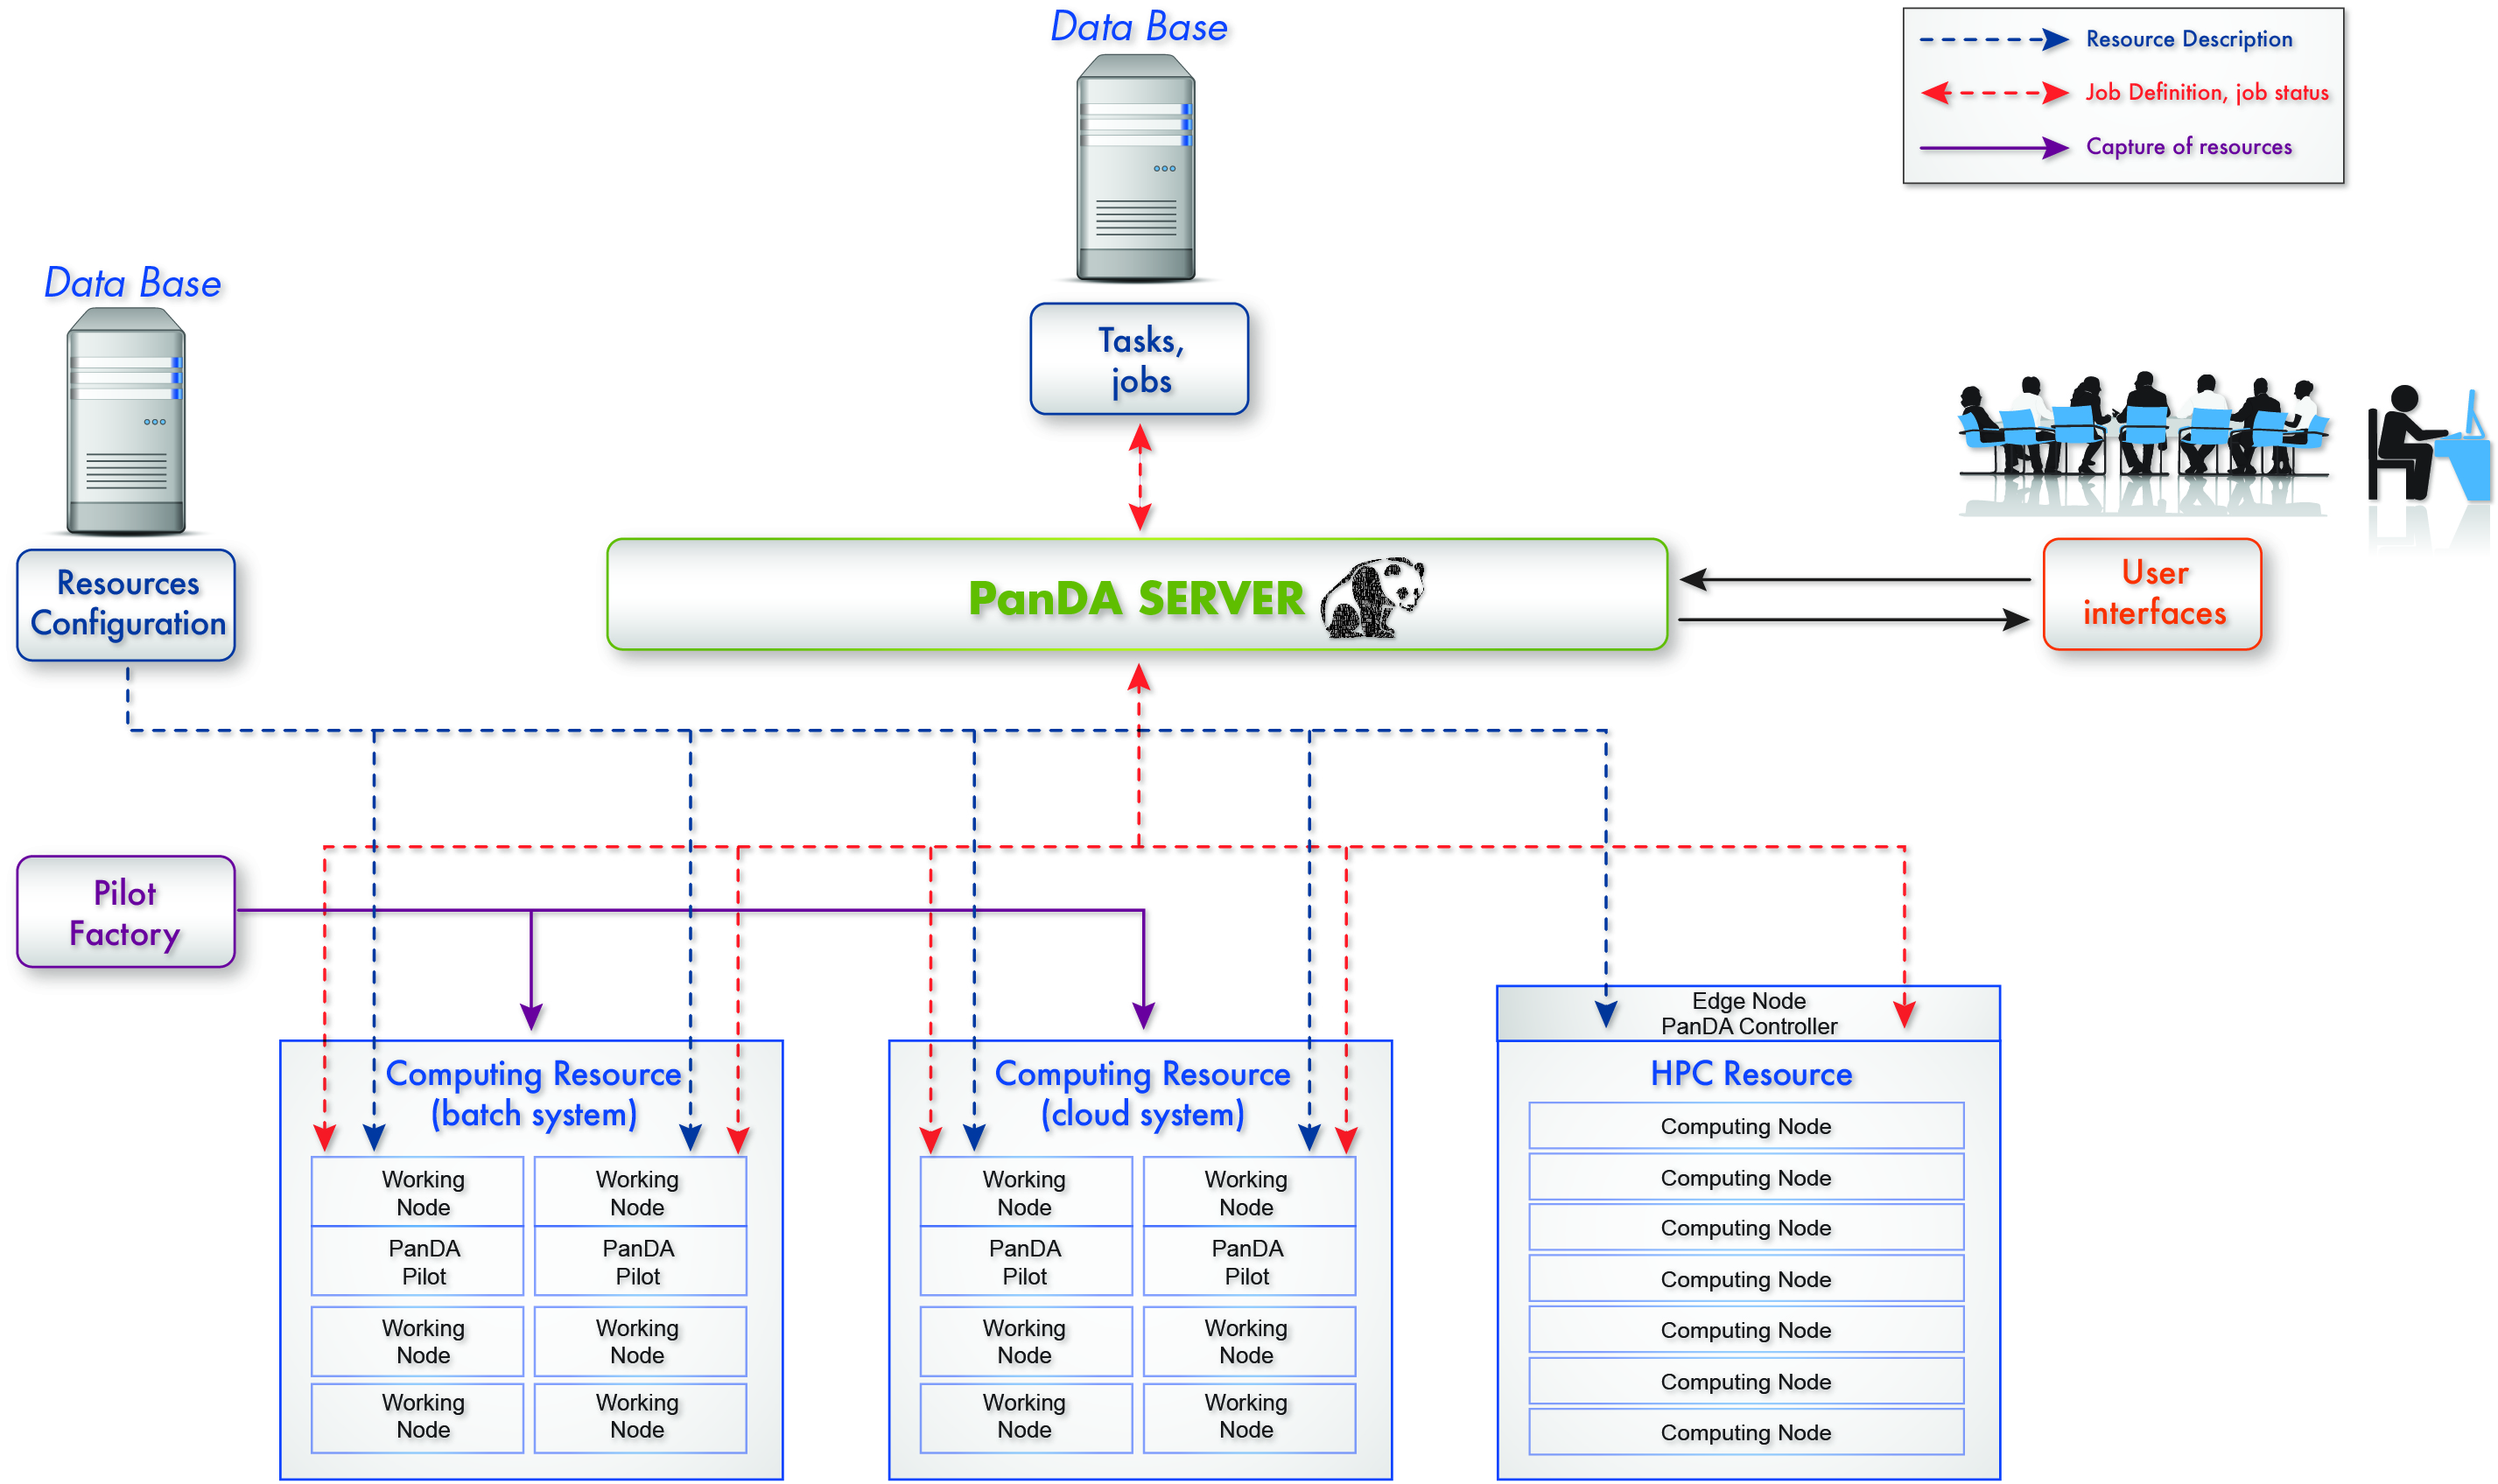
\includegraphics[width=\columnwidth]{figures/PandaArch.jpg}
  \end{center}
\caption{\mtnote{This diagram is a placeholder. I am working on a substitute
that will be referenced when describing PanDA's subsystems.}Schematic view of
the PanDA system, as deployed for production in 2017. Black boxes indicate
PanDA's subsystems; Orange boxes components of a subsystem; purple boxes
databases; green arrows http messaging interfaces; red arrows API; purple arrows
database communications.}
% Originally PanDA was designed for grid infrastructure... In this
% paper is focussed on the HPC use case; there are differences from
% the grid use case. This paper discusses how PanDA has been adapted
% to execute a workload % on HPC resources. The schematic overview is
% presented for workload X on Titan......
\label{fig:architecture}
\end{figure}

\paragraph{\textbf{PanDA Server}} this subsystem is the central hub service of
PanDA and it operates as a web service. It runs on Apache web server,
interacting with the back-end database running on separate servers. It
implements the Apache worker model, with many independent processes handling
client requests in parallel. Since all state is maintained in the central
database, the PanDA Server application instance itself is stateless. Currently
production version of PanDA utilizes Oracle database backend, but PanDA can also
work with MySQL family of databases.

% . It provides a task queue
% managing all job information centrally. The PanDA server receives jobs through
% the client interface into the task queue, upon which a brokerage module
% operates to prioritize and assign work on the basis of job type, priority,
% input data and its locality, and available CPU resources. The PanDA server

PanDA Server implementation consists of four components, all implemented in
Python and communicating via Python APIs: Task Buffer, Brokerage, Job
Dispatcher, and Data Service. Task Buffer is the management component of PanDA's
global queue and offers functionalities to: (i) store jobs into the global
queue; (ii) provide information about and update the state of each stored job.
The Brokerage component enables (i) matching job attributes with site and pilot
attributes; (ii) managing the dispatch of input data to processing sites; and
(iii) deriving PanDA's data pre-placement requirement.
% The job/pilot matching algorithm assigns a weight to each candidate pilot and
% after applying a set of policies, the best ten candidates are taken.
The Job Dispatcher implements functionalities to: (i) receive requests from
active pilots for new jobs to process; (ii) retrieving from Task Buffer the jobs
with highest priority that can be executed on the resource on which the
requesting pilots have been instantiated; (iii) creating a wrapper for the
selected job, tailored to the resource of the requesting pilot; and (iv)
monitoring the state of the job execution on the pilot, updating the Task Buffer
component. Finally, the Data Service component offers functionalities to: (i)
retrieve information from Task Buffer and Brokerage about the data requirements
of each job and the resource to which each job has been assigned; (ii) enable
interaction with the ATLAS DDM to make input files available to the jobs and
manage their output data.

\paragraph{\textbf{PanDA Pilot}} this subsystem implements the execution
environment for PanDA's jobs. Implemented in Python, a PanDA Pilot is launched
by a wrapper submitted to a site. Wrappers are tailored to the
specific interfaces and middleware exposed by each site so that PanDA Pilot
remains site-independent. PanDA Pilot implements four main functionalities: (i)
preparing the execution environment for PanDA's jobs,
% including  recovering and cleaning up previously failed jobs on that site and
collecting information about the compute, data, and network capabilities of the
site; (ii) requesting a job for execution to the Job Dispatcher component of
PanDA Server; (iii) initiating and monitoring the execution of pulled jobs,
including setting up the job, transferring its input when required, executing
the payload, transferring output, and checking log files and local space; and
(iv) clean up when the payload has finished to execute.

% PanDA is a pilot based workload management system.
% In the PanDA job lifecycle, pilot jobs (Python scripts that organize workload
% processing on a worker node) are submitted to sites. When these pilot jobs
% start on a worker node they contact a central server to retrieve a real
% payload (i.e., an end-user job) and execute it.

PanDA Pilot implements the pilot paradigm~\cite{pilot_review}, decoupling
resource acquisition from job execution via multi-stage scheduling. This has
several benefits, including increasing throughput by lowering the time taken to
queue and schedule jobs; enabling both concurrent and sequential job execution
depending on the number of cores available to the pilot and the time for which
it remains available; and exposing a unified and consistent interface for the
scheduling of jobs, independent from the middleware of the site on which the
pilot has been instantiated.

% The specific implementation of PanDA Pilot promotes reliability by
% monitoring the execution of the job's payload, and a certain degree of
% fault-tolerance by recovering information and, possibly, output files from
% jobs that failed, even before instantiating the PanDA Pilot.

% Using these pilot-based workflows helps to improve job reliability, optimize
% resource utilization, allows for opportunistic resources usage, and mitigates
% many of the problems associated with the inhomogeneities found on the Grid.

It should be noted that upon bootstrapping, a PanDA Pilot download major parts
of its runtime code via HTTP from a central Subversion repository. The
repository works with an Apache web server, configured with a memory-based web
proxy (Squid). The purpose of the cache is to reduce the request load on the
back-end Subversion server. That improves performance \mtnote{Do we have
data/numbers?} since only occasional queries trigger a full lookup on the
back-end Subversion system, and most external queries are pulled from memory on
the front-end web server. The benefits of this system include a high-performance
code download service, combined with code updates still being immediately
available as soon as they are committed to source code control.

\paragraph{\textbf{AutoPyFactory}} this subsystem implements a factory to submit
pilots locally and to both grid and cloud
sites~\cite{caballero2012autopyfactory}. Implemented to be executed as a single
demonized process, AutoPyFactory enables the concurrent spawning of multiple job
submission processes called APFQueue. Each APFQueue can communicate with PanDA
Server and the Brokerage module to collect information about the state of the
jobs it manages and, on the base of this information, submit new pilots to one
site per APFQueue. AutoPyFactory implements functionalities to evaluate the
number of pilots already instantiated on each site, and to apply a consistent
and adequate pressure on their batch queues. Submission is performed via the
Condor-G batch system~\cite{frey2002condor}, enabling submission to multiple
type of sites. AutoPyFactory exposes a dedicated monitoring service, feeding
information to the PanDA Monitoring subsystem. A proxy manager is also run,
enabling certificate-based authentication and authorization.

% As a pilot-based system, PanDA requires some way to get the initial PanDA
% pilot onto worker nodes at sites. This is done with the help of a component
% called AutoPyFactory (APF). APF runs in a single daemonized process,
% launching a separate thread for each internal workflow. Each one of these
% internal workflows typically serves a single job queue as defined in WMS, and
% delivers pilots to a single batch queue, either local or remote. The behavior
% of these APF workflows is determined by the combination of a set of plugins,
% invoked in a fixed order, in a loop, each one in charge of the performance of
% a well defined action.

\paragraph{\textbf{PanDA Monitoring}} this subsystem is implemented as a
web-based, dashboard-style graphical application~\cite{klimentov2011atlas}. It
runs on Apache and interacts with the back-end database of PanDA Server to
enable persistence. PanDA Monitoring enables users and site administrators to
gather information about the status of current and past jobs, data movement, and
pilot factory. PanDA Monitoring allows users access to all log files of each
job, greatly simplifying code debugging and failure analysis in a distributed
computing environment.

\paragraph{\textbf{JEDI}} this subsystem implements a workload and workflow
management for tasks instead of jobs, as defined by HEP
users~\cite{borodin2015scaling}. Implemented as a standalone service that
interacts with Panda Server via its REST interface, JEDI offers two main
functionalities: partitioning tasks to jobs, and binding jobs to resources via
dedicated queues. JEDI partition tasks to jobs by matching tasks requirements to
resource capabilities. This matching is based on tasks attributes, and static
and dynamic information about the resources of each available site. Dynamic
information is acquired via a small number of `scout' jobs that collect
information about current resources and their performance. Functionally, JEDI
defines a set of queues associated to groups of resources with specific
capabilities. Tasks are assigned to groups of these queues, and the jobs in
which each task is partitioned are assigned to each queue, depending on their
requirements. JEDI replaces the job brokerage functionalities of the Brokerage
module of the PanDA Server but this module still handles communication between
the Task Buffer and the Data Service modules.
%, using it to enact the execution of the jobs defined by JEDI
% on the resources and sites decided by JEDI.


% -----------------------------------------------------------------------------
\subsection{Execution}
\label{ssec:panda_exec}

% The tasks of workloads and workflows submitted to PanDA are partitioned
% to one or more jobs. Each job is then executed on one of the available
% PanDA Pilots, chosen among those that the PanDA Server manages across multiple
% sites. Tasks processes a certain amount of events that are stored into files,
% and when a task is partitioned to multiple jobs, subsets of events need to be
% assigned to each job and made available to the pilot on which that job will be
% executed. Finally, the output of each job need to be retrieved and aggregated
% into the output of the original task (Fig.~\ref{fig:architecture}).

The relation between tasks and jobs can be one-to-one or one-to-many, and the
conversion between the two can by static or dynamic. During the LHC Run 1, PanDA
required users or the application layer to perform a static conversion between
tasks and jobs: tasks were described as a set of jobs with a fixed number of
events and then submitted to the PanDA Server (Fig.~\ref{fig:architecture}:A1).

This approach introduced inefficiency both with usability and resource
utilization~\cite{borodin2015unified}. Ideally, users should not have to reason
in terms of jobs: Users conceive analyses in terms of one or more, possibly
related tasks; the `job' abstraction is required exclusively by the execution
middleware, i.e. PanDA. Further, a static partitioning of tasks into jobs does
not take into account the heterogeneity and dynamicity of the resources of the
pilots on which each job will be executed.

Another problem of static job sizing is that PanDA instantiates pilots on sites
with different type of resources and different models of availability of those
resources. An optimal sizing of each job should take into account these
properties. For example, sites may offer cores with different speed, networking
with different amount of bandwidth, and resources could be guaranteed to be
available for a defined amount of time or could disappear at any point in time
as with opportunistic models of resource provision.

JEDI was deployed for the LHC Run 2 to address these inefficiencies with a
machine-driven conversion of tasks into jobs. Users or the application layer (i)
submits tasks descriptions to JEDI; (ii) JEDI partitions tasks to jobs of
different size, depending on both static and dynamic information about available
resources; (iii) jobs are bound to sites with resources that best match jobs'
requirements; and (iv) jobs are submitted to the PanDA Server for execution
(Fig.~\ref{fig:architecture}:A2-B).

Once submitted to the PanDA Server, jobs are stored by the Task Buffer component
into a global queue implemented as a relational database
(Fig.~\ref{fig:architecture}:C). When jobs are submitted directly to the PanDA
Server, the Brokerage component is used to bind jobs to available sites,
depending on static information about the resources available for each site.
Jobs submitted by JEDI are instead already bound to resources so no further
brokerage is needed. Once jobs are bound to sites, the Brokerage module
communicates to the Data Service module what data sets need to be made available
on what site. The Data Service communicates these requirements to the ATLAS DDM
that, when needed, takes care of aggregating files into datasets and containers,
replicating them on the required sites.

The AutoPyFactory subsystem communicates with the Task Buffer component of the
PanDA Server, acquiring information about jobs that have been bound and are
ready for execution. On the base of this information, AutoPyFactory defines a
set of suitable PanDA Pilots, queues them into APFQueues, and concurrently
submits them to multiple sites.

% AutoPyFactory submits pilots only when similar pilots are not yet available
% and maintains a predefined amount of pressure on the queue of each site. In
% this way, resource availability and utilizations is optimized.

When PanDA Pilots become available on sites, they
% bootstrap, download their code, collect information about the execution
% environment and
call the Job Dispatcher module of the PanDA Server, requesting for a job to
execute \mtnote{Can a pilot request multiple jobs to execute
concurrently?}\sergeynote{In principle it should be able to do that, but that's not
how it is operated. One pilot - one job is a cleaner model in an environment
where resources are "owned" by the organization that runs pilots. Simplifies
many things. At least as far as I know.}. The Job Dispatcher communicates with
the Task Buffer, requesting for a job that is bound to the site of that pilot
and ready to be executed. Task Buffer checks the global queue (i.e., the PanDA
database) and if such a job is available, it passes the job handler to the Job
Dispatcher. The Job Dispatcher dispatches the job to the PanDA Pilot.

Upon receiving a job, a PanDA Pilot starts a monitoring process and forks a
subprocess for the execution of the job's payload. The job is setup, input data
are transferred from the designated staging in location, and the job's payload
is executed. Once completed, output is transferred to the staging out location.
% During the job's payload execution, the monitoring process of PanDA Pilot
% checks the status of the job execution and its environment.

The Data Service module of the PanDA Server tracks and collects the output
generated by each job, updating jobs' attributes via the Task Buffer module.
When the output of all the jobs of a task are retrieved, they are aggregated and
made available to the user either via the PanDA Server of the JEDI service,
depending on how tasks or jobs were initially submitted.

\mtnote{Think whether a comparison with other WMS based on the review we did
makes sense in this context.}\sergeynote{You provided a nice description of the
PanDA system here.}
